\section{Model Predictive Control}
\label{sec:ModelPredictiveControl}
In this section we explain the basis of MPC, the cost function used for optimizing, and an efficient algorithm to implement the control.

Model predictive control is an optimal control technique mainly used to solve control problems in presence of constraints. These constraints can represent physical capabilities of the controlled system, like the steering angle of a vehicle or its acceleration, or restrictions/requirements of the control problem that is being solved, like the road boundaries that the vehicle is not allowed to cross or its desired maximum orientation angle.

\subsection{Mathematical Formulation}
\begin{subequations}\label{eq:MathematicalFormulation}
\begin{align}
U_t^*(x(t)) = \argmin_{U_t}&\sum\limits_{k=0}^{N-1}q(x_{t+k},u_{t+k}) \\
  \text{s.t.} \quad &x_t = x(t) \\
  &x_{t+k+1}  = Ax_{t+k}+Bu_{t+k},~\forall k\geq 0 \\
  &x_{t+k} \in \mathcal{X},u_{t+k} \in \mathcal{N},~\forall k\geq 0 \\
  &U_t = \{u_t,u_{t+1},\ldots,u_{t+N-1}\}
\end{align}
\end{subequations}
Problem is defined by \\
\indent $\blacksquare$ Objective that is minimized \\
\indent $\blacksquare$ Internal system model to predict system behavior \\
\indent $\blacksquare$ Constraints that have to be satisfied \\
\subsection{Length and duration}

The prediction horizon is the duration over which future predictions are made. We’ll refer to this as T.
T is the product of two other variables, N and dt.
N is the number of timesteps in the horizon. dt is how much time elapses between actuations. For example, if N were 20 and dt were 0.5, then T would be 10 seconds.
N, dt, and T are hyperparameters you will need to tune for each model predictive controller you build. However, there are some general guidelines. T should be as large as possible, while dt should be as small as possible.

These guidelines create tradeoffs.

\noindent{\bf Horizon} \\
In the case of driving a car, T should be a few seconds, at most. Beyond that horizon, the environment will change enough that it won't make sense to predict any further into the future.

\noindent{\bf Number of Timesteps} \\
The goal of Model Predictive Control is to optimize the control inputs: [$\delta$,a]. An optimizer will tune these inputs until a low cost vector of control inputs is found. The length of this vector is determined by N:
\[
  % [\delta_1,a_​1, \delta_2,a_2,...,\delta_{N−1},a_{​N−1}]
  [\delta_1,a_​1, \delta_2,a_2,\ldots,\delta_{N−1},a_{​N−1}]
​​\]

Thus N determines the number of variables optimized by the MPC. This is also the major driver of computational cost.

\noindent{\bf Timestep Duration} \\
MPC attempts to approximate a continuous reference trajectory by means of discrete paths between actuations. Larger values of dt result in less frequent actuations, which makes it harder to accurately approximate a continuous reference trajectory. This is sometimes called ``discretization error".

A good approach to setting N, dt, and T is to first determine a reasonable range for T and then tune dt and N appropriately, keeping the effect of each in mind.

\subsection{Coordinate transformation}
The simulator returns waypoints using the map's coordinate system, which is different than the car's coordinate system. Transforming these waypoints will make it easier to both display them and to calculate the CTE and $e_{\psi}$ values for the model predictive controller.

Since the simulator speed is in mph and the latency is measured in seconds. So the speed from simulator and the reference speed should be converted to m/s before feeding the solver.

\begin{lstlisting}[label={list:list1},language=C++,caption=Car's coordinate transform.]
h.onMessage([&](uWS::WebSocket<uWS::SERVER> ws, char *data, size_t length, uWS::OpCode opCode) {
          ......

          vector<double> next_x_vals;
          vector<double> next_y_vals;

          Eigen::VectorXd car_x_vals(ptsx.size());
          Eigen::VectorXd car_y_vals(ptsy.size());
          for (int i = 0; i < ptsx.size(); ++i) {
            double dx = ptsx[i] - px;
            double dy = ptsy[i] - py;
            car_x_vals[i] = cos(-psi) * dx - sin(-psi) * dy;
            car_y_vals[i] = sin(-psi) * dx + cos(-psi) * dy;

            next_x_vals.push_back(car_x_vals[i]);
            next_y_vals.push_back(car_y_vals[i]);
          }

          ......
}

\end{lstlisting}

\subsection{Latency}

A safe control system requires sophisticated methods to handle the latency or delays brought by both the vehicle’s mechanical system and the communications systems.

A contributing factor to latency is actuator dynamics. For example the time elapsed between when you command a steering angle to when that angle is actually achieved. This could easily be modeled by a simple dynamic system and incorporated into the vehicle model. One approach would be running a simulation using the vehicle model starting from the current state for the duration of the latency. The resulting state from the simulation is the new initial state for MPC.

The both implementations can handle latency very well, the MPC can process latency either before or after the vehicle coordinate system transform.

\begin{lstlisting}[label={list:list2},language=C++,caption=Handle latency after car's coordinate transform.]
h.onMessage([&](uWS::WebSocket<uWS::SERVER> ws, char *data, size_t length, uWS::OpCode opCode) {
          ......

          double dt = 0.1;
          px = 0;
          py = 0;
          psi = 0;
          double cte  = polyeval(coeffs, 0.0);
          double epsi = -atan(coeffs[1]);

          px = px + v * cos(psi) * dt;
          py = py + v * sin(psi) * dt;
          const double Lf = 2.67;
          psi = psi + v * delta / Lf * dt;
          v = v + a * dt;
          cte = cte + v * sin(epsi) * dt;
          epsi = epsi + v * delta / Lf * dt;

          Eigen::VectorXd state(6);
          state << px, py, psi, v, cte, epsi;

          auto vars = mpc.Solve(state, coeffs, weights);
          ......
}

\end{lstlisting}

\begin{lstlisting}[label={list:list3},language=C++,caption=Handle latency before car's coordinate transform.]
h.onMessage([&](uWS::WebSocket<uWS::SERVER> ws, char *data, size_t length, uWS::OpCode opCode) {
          ......

          double dt = 0.1;
          px = px + v * cos(psi) * dt;
          py = py + v * sin(psi) * dt;
          const double Lf = 2.67;
          psi = psi + v * delta / Lf * dt;
          v = v + a * dt;

          Eigen::VectorXd state(6);
          state << px, py, psi, v, cte, epsi;

          auto vars = mpc.Solve(state, coeffs, weights);
          ......
}

\end{lstlisting}

\subsection{Polynomial fit}
We approximate $X_{ref}$ and $Y_{ref}$ over the next planning horizon $T$ as third order polynomials of the curvilinear position, starting at the point closest to the vehicle's current position.

\subsection{Cost function}
% A cost function is a performance index which is minimized or maximized. There are several types of cost function, the most basic ones are the Time Optimal, which only penalize the time that takes to a system to go from one point to another, the Minimum-Effort, which minimize the effort or cost of a process and the General Optimal Control, which is the most used as it can represent any problem with the suitable functions and it can be defined in a quadratic form

The way to define the cost function used in this problem, once discretized and taking into account the prediction and control horizons is the one shown in equation \eqref{eq:CostFunction}

\begin{equation}\label{eq:CostFunction}
\begin{aligned}
  J & = \sum\limits_{t=0}^{N}(w_{cte}(cte_t-cte_{ref})^2 + w_{\psi}(e_{\psi_t}-e_{\psi_{ref}})^2 + w_v(v_{t}-v_{ref})^2) \\
    & + \sum\limits_{t=0}^{N-1}(w_{\delta}\delta_t^2 + w_aa_t^2) \\
    & + \sum\limits_{t=0}^{N-2}(w_{\dot{\delta}}(\delta_{t+1}-\delta_t)^2 + w_{\dot{a}}(a_{t+1}-a_t)^2)
    % & + \sum\limits_{t=0}^{N-2}(w_{\Delta \delta}(\delta_{t+1}-\delta_t)^2 + w_{\Delta a}(a_{t+1}-a_t)^2)
\end{aligned}
\end{equation}

\subsection{Constraints}

One of the obvious constraint to define is the restriction of the vehicle to not pass the road boundaries. It is desired to set the middle of the lane as $cte = 0 ~\small{m}$. Another constraint to define for security reasons and for the capabilities of the vehicle motor is the velocity, steering angle and acceleration. The velocity cannot be negative and it is capped at $v_{max} \approx 29 ~\small{m / s}$ and regarding the acceleration it is capped at $-1~\small{m/s^2} \leq a  \leq ~\small{1m/s^2}$. For comfort reasons, the steering angle  ($\delta$) variations have also been constrained with values of $-25\degree \leq  \delta \leq 25\degree$


\subsection{Tuning parameters}


The parameters that have to be tuned for the controller to work as good as possible are the prediction horizon N, the weights, as well as the sampling time. First of all the number of timesteps(N) and the timestep duration(dt) have to be chosen such that $N*dt \approx 1.5~\small{seconds}$. In the case of driving a car, T should be a few seconds, at most. Beyond that horizon, the environment will change enough that it won't make sense to predict any further into the future. However, the choice of N will influence the number of variables̄, which is the major driver of computational cost.

Since the prediction horizon does not affect the other parameters, the tuning of the horizon length N is less involved. The only requirement is that the optimization problem should be feasible. Thus, it becomes clear that the horizon length will be dependent on the sampling distance, which can be achieved for multiple combinations of sampling time and speed. If the sampling distance is short, a longer horizon will be needed, and vice versa. In short, it is desirable to keep N small for computational reasons, but on the other hand it has to be suffciently large for the problem to be feasible.

This article recommends tuning the weights on the inputs as well as the rate of change of the inputs. Penalizing the rate of change yields a more robust controller but at the cost of the controller being more sluggish. Setting a small penalty or none whatsoever gives a more aggressive controller that is less robust. For instance, tuning weight of the steering value in the cost function results in a smoother steering transitions.

Here are my final hyperparameters shown in table~\ref{table:hp}, The hyperparameters are used in the nominal optimal control problem meaning that the mangnitude of lateral control (steering) are penalized more than longitudinal control (throttle and brake).

\begin{table}[h!]
\centering
\scalebox{0.9}{
\begin{tabular}{| c | c | c | c | c | c | c | c | c | c | c |}
\hline
{model and latency} & {$N$} & {$dt$} & {$v$} & {$w_{cte}$} & {$w_{\psi}$} & {$w_{v}$} & {$w_{\delta}$} & {$w_{a}$} & {$w_{\dot{\delta}}$} & {$w_{\dot{a}}$} \\
\hline
kinematic - 100 ms & 10  & 0.15  &$29~\small{m/s}$ & 1.0 & 1.0 & 1.0 & 1000.0 & 1.0 & 500.0 & 1.0 \\
\hline
\end{tabular}
}
\vspace{0.1cm}
\caption{Final hyperparameters.}
\label{table:hp}
\end{table}

\begin{figure}[H]
\centering
    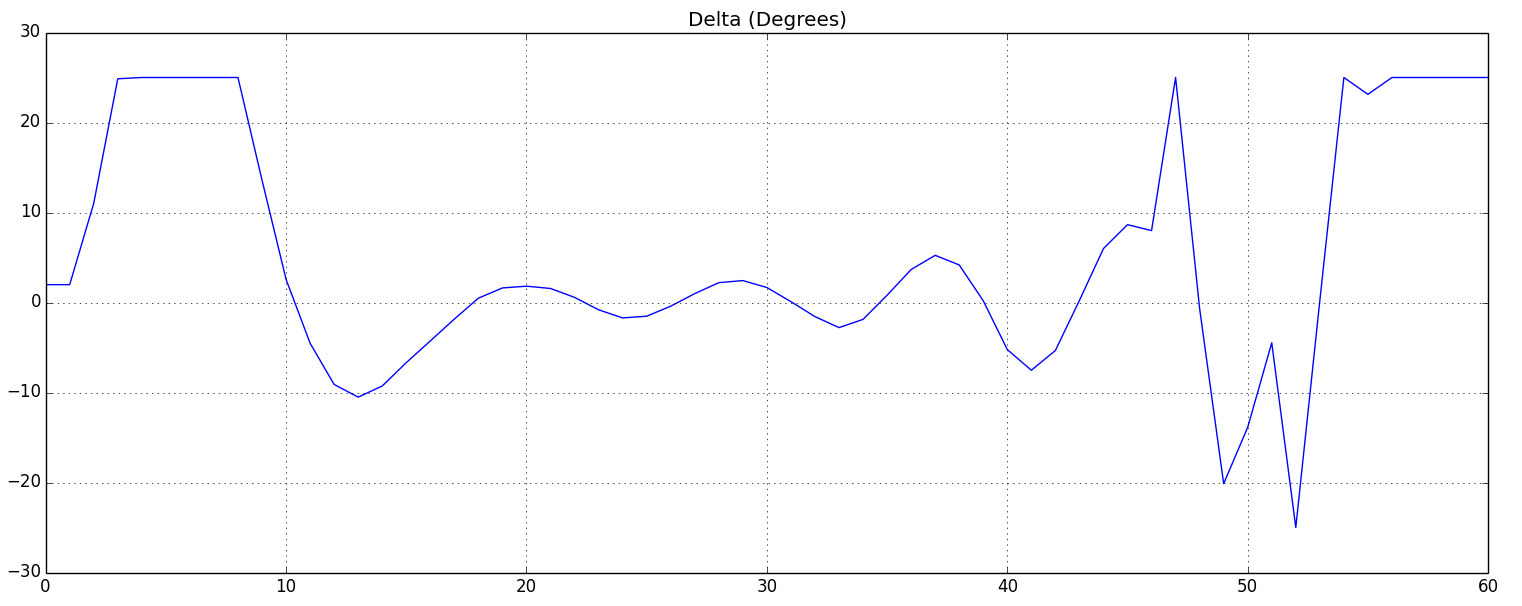
\includegraphics[width=0.8\linewidth]{./delta_1_100.png}
      \vspace{-0.1cm}
\caption{$w_{\delta}=1$ $w_{\dot{\delta}}=100$}
\label{fig:fig1}
\end{figure}

\begin{figure}[H]
\centering
    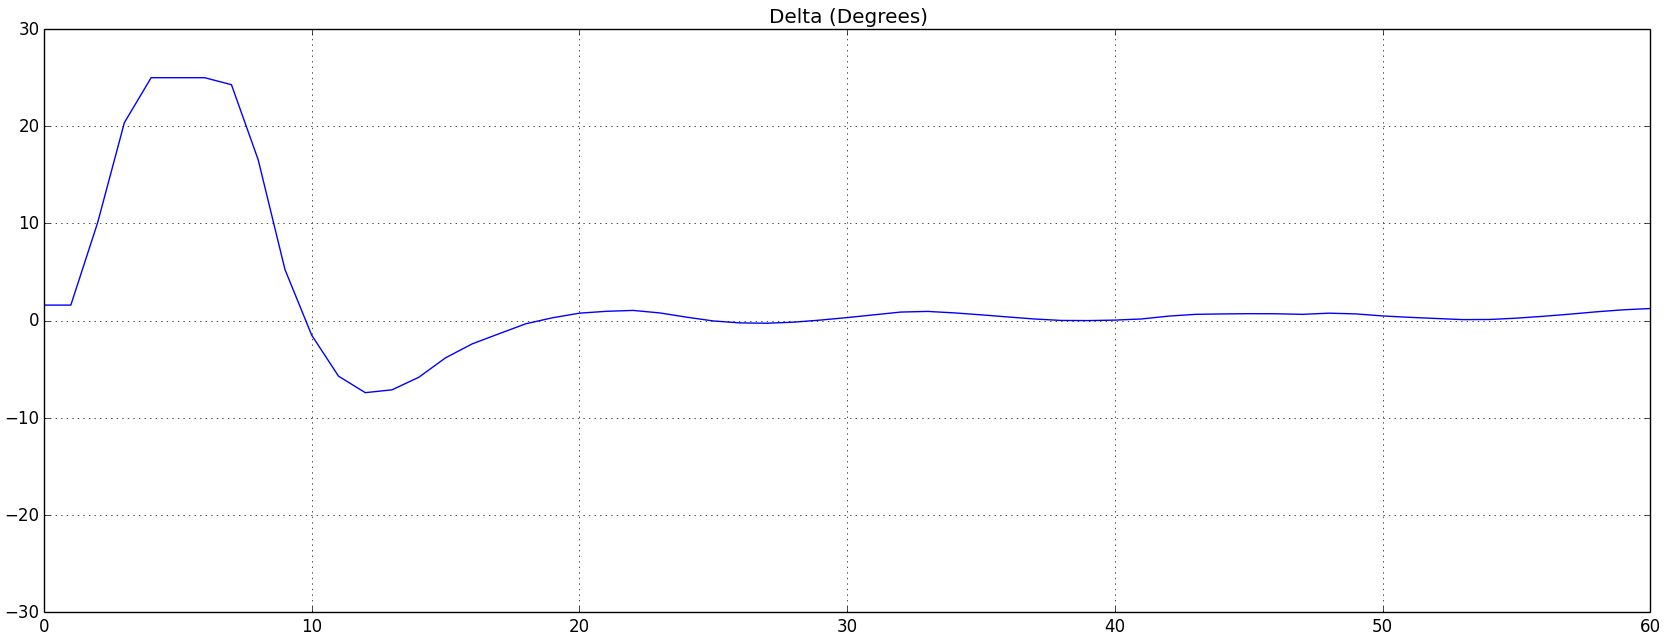
\includegraphics[width=0.8\linewidth]{./delta_1_500.png}
      \vspace{-0.1cm}
\caption{$w_{\delta}=1$ $w_{\dot{\delta}}=500$}
\label{fig:fig2}
\end{figure}

\begin{figure}[H]
\centering
    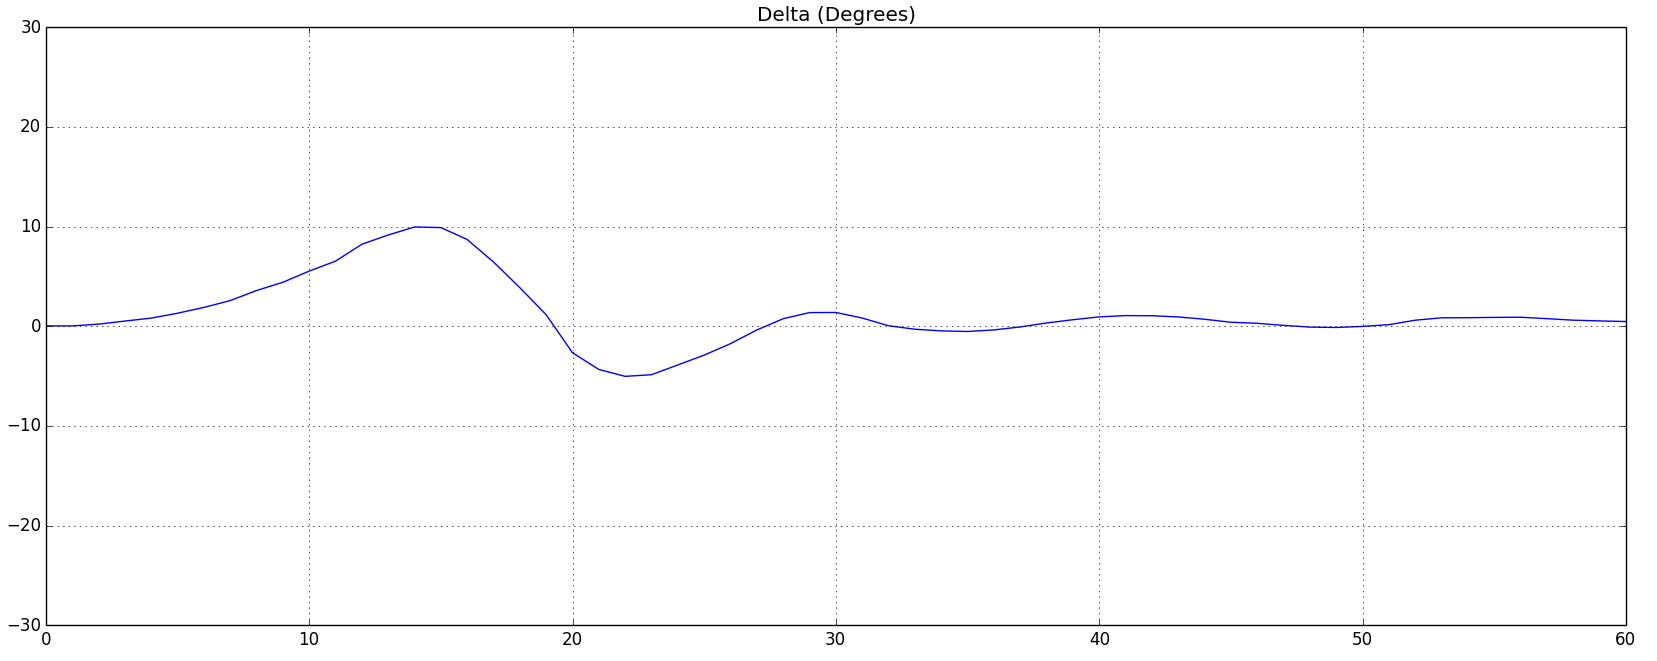
\includegraphics[width=0.8\linewidth]{./delta_50_500.png}
    \vspace{-0.1cm}
\caption{$w_{\delta}=50$ $w_{\dot{\delta}}=500$}
\label{fig:fig3}
\end{figure}

As we can see increasing weight of the steering value in the cost function results in a smoother steering transitions.

\begin{figure}[H]
\centering
    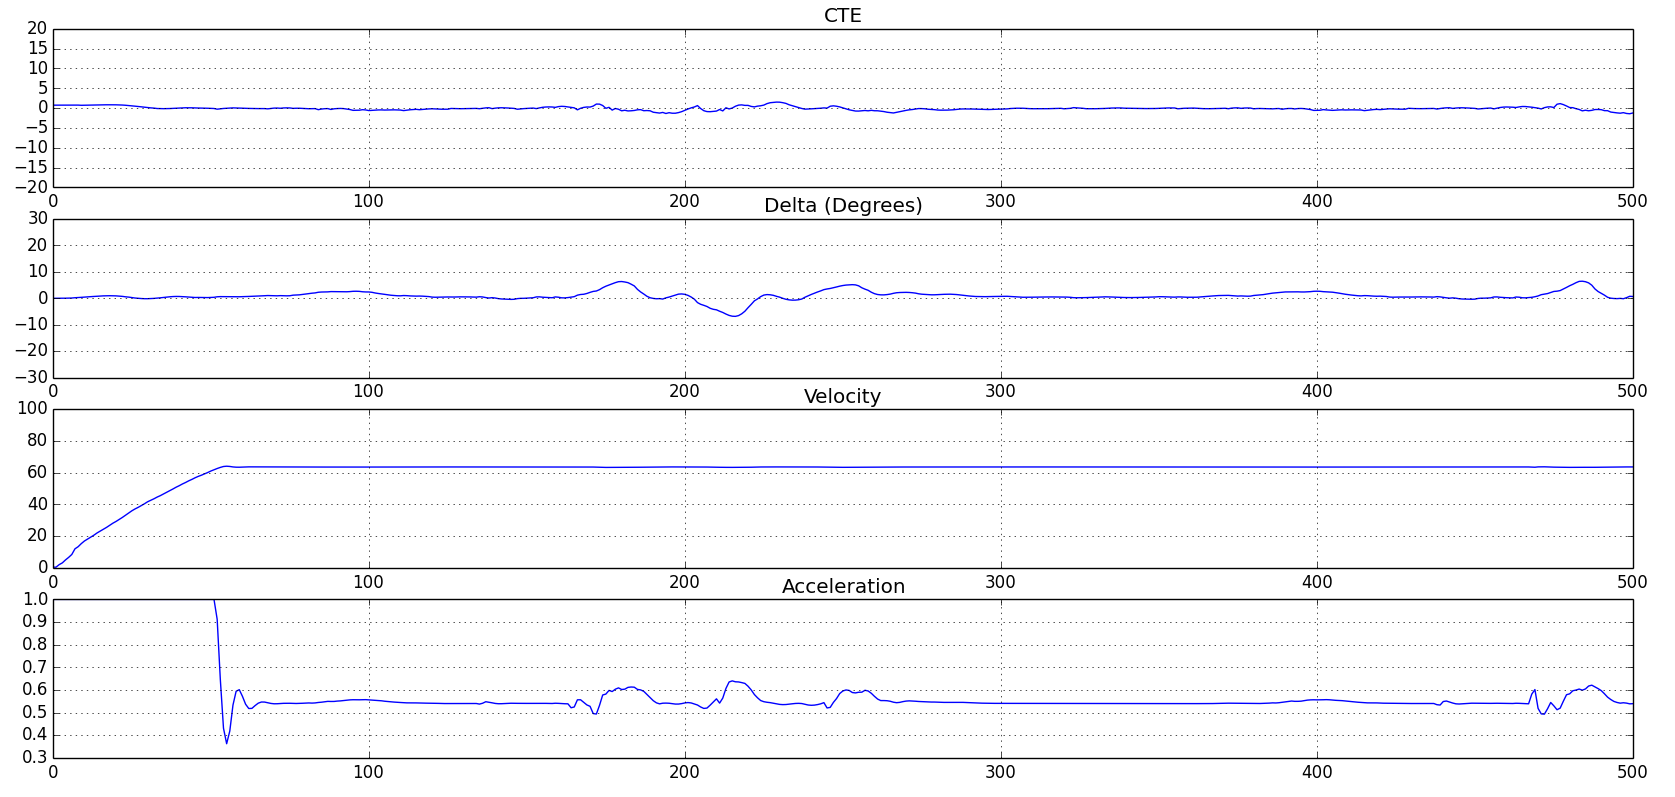
\includegraphics[width=0.8\linewidth]{./figure4.png}
      \vspace{-0.1cm}
\caption{$N=10$ $dt=0.15$}
\label{fig:fig4}
\end{figure}
